\chapter{Reconstrucci\'on tomogr\'afica en radiodiagn\'ostico}

En este capítulo se presentarán los fundamentos matemáticos sobre los cuales se sostiene la reconstrucción tomográfica para obtener cortes transversales a partir de imágenes radiográficas. Posteriormente se presentarán las características necesarias para el haz de irradiación y los diferentes parámetros en la adquisición de imágenes de CT\footnote{Tomografía Computada, por sus siglas en inglés ``\emph{Computed Tomography}''}, así como aplicaciones en radiodiagnóstico anatomico y metabólico y el procesamiento de imágenes 3D.

\section{Introducci\'on}

El concepto -y la palabra- tomografía proviene de la conjunción de dos palabras griegas: $\tau o \mu o \varsigma$ ('tomos': corte, rebanada) y $\gamma \rho \alpha \varphi \omega$ ('grafo': escribir). La técnica consiste en la adquisición de imágenes resultantes de la atenuación de un haz de rayos X al atravesar un cuerpo desde diferentes ángulos, y por medio de la implementación de modelos matemáticos que permiten reconstruir las estructuras internas del mismo para obtener cortes transversales y una imagen tridimensional del cuerpo en función de las propiedades de absorción de rayos X de sus materiales.

En el proceso, los rayos X son producidos en un tubo de rayos X, son atenuados por el cuerpo al que se le realiza la irradiación y detectados por un detector de rayos X, esto produce una ``proyección''. Este proceso es repetido para diferentes ángulos de irradiación y por medio de métodos de reconstrucción tomográfica, con estas proyecciones se obtienen los cortes transversales que dan lugar a la imagen 3D.

En 1917, Radon postula las bases matemáticas para la obtención de cortes transversales a partir de proyecciones, dando lugar a la conocida ``Transforma de Radon''. Recién en 1971 se construye el primer equipamiento que utiliza este tipo de tecnología a partir de imágenes de rayos X (descubiertos por Röntgen en 1895), el cual es presentado en 1972 en Inglaterra por parte de Hounsfield. Esto le valió el Premio Nobel de Fisiología o Medicina en 1979.

Las imágenes de CT consisten principalmente de tensores de dimensión $n\times m \times l$ donde los cortes transversales son representados por matrices $n\times m$ y $l$ representa el número de cortes transversales. Los niveles de grises de las imágenes son presentados en ``unidades de Hounsfield'' ($HU$, por sus siglas en inglés), definidas a partir del coeficiente de atenuación del agua, $\mu_{H2O}$.

\begin{equation}
 \text{Número de CT (en $HU$)} = \frac{\mu - \mu_{H2O}}{\mu_{H2O}} \cdot 1000
\end{equation}

\noindent
donde $\mu$ es el coeficiente de atenuación lineal de los materiales del cuerpo. Así, los $HU$ de agua y aire resultan 0 y -1000, respectivamente, mientras que le hueso y materiales más densos\footnote{Nótese que en este contexto el concepto de ``densidad'' se refiere a la densidad electrónica, que define las propiedades de atenuación del haz de rayos X.} que el agua dan por resultado $HU > 0$.

\section{Tipos de scaner CT}

La historia de los escáneres de CT data, como se menciona antes, de 1971 con el desarrollo del primer equipamiento presentado por Hounsfield. Estos escáneres evolucionaron tanto desde el punto de vista técnológico como de los métodos para la obtención de las proyecciones y son consecuente reconstrucción tomográfica. El primer tipo de escáner contemplaba un arreglo geométrico de haz paralelo, creándose el primero de haz en forma de abanico (\emph{fan-beam}) en 1976. Recién en 1989 surge el primer escáner que obtiene imágenes girando el sistema tubo-detectores de forma contínua y sincronizada con el movimiento de la mesa donde se ubica el paciente, dando lugar a la adquisición de tipo helicoidal o espiral y posteriormente a la adquisición de varios cortes para un mismo giro.

La figura \ref{fig:10-0.1} muestra una línea del tiempo con los distintos tipos de escáneres de CT y el avance tecnológico.

\begin{figure}
 \centering
 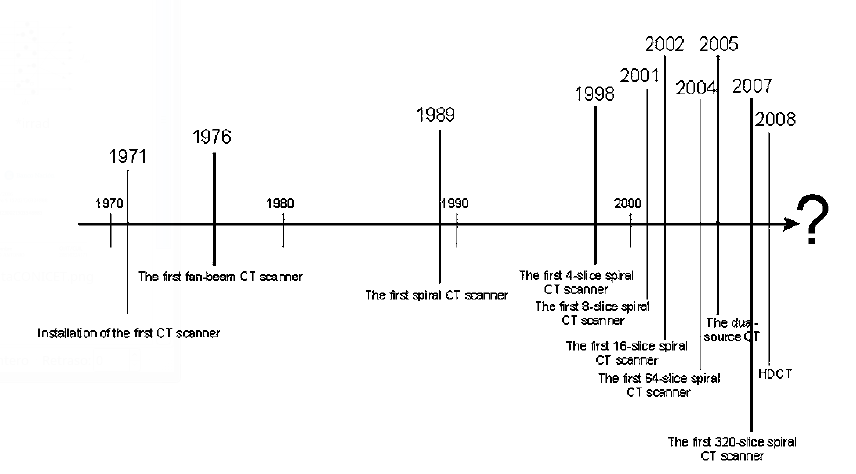
\includegraphics[width=.75\textwidth]{Figuras/fig10-01.png}
 \caption{Imagen tomada del libro \emph{X-Ray Computed Tomography in Biomedical Engineering}.}
 \label{fig:10-0.1}
\end{figure}

Una forma de clasificar los diferentes tipos de escáners, su método de adquisición de proyecciones y sus tipos de reconstrucción se puede definir en función de 3 diferentes tipos de configuración:

\begin{itemize}
 \item Sistema de proyección utilizando haz paralelo
 \item Sistema de proyección utilizando \emph{fan-beam}
 \item Sistema de proyección utilizando haz cónico (\emph{cone-beam})
\end{itemize}

El sistema de proyección utilizado, y la configuración de las diferentes partes del escáner (gantry, tubo de rayos X, arreglo de detectores y mesa) define los escáneres en función de su generación.

\subsection{1era generaci\'on}

Los escáneres de primera generación (1971) también conocidos como \emph{pencil beam} o \emph{traslational/rotational single detector} son aquellos que contemplan el uso de un haz paralelo y dos tipos de movimiento del gantry. Un movimiento lateral contínuo, para el cual el gantry se mueve de forma contínua en $z$ para la obtención de datos para un determinado ángulo, y un sistema de rotación circular discreta donde se obtienen las proyecciones para cada ángulo.

En los escáneres de primera generación el movimiento lateral puede ser contínuo o discreto, mientras que el movimiento circular es siempre discreto. Cada proyección se construye con un ``ida y vuelta'' en movimiento lateral para cada ángulo fijo.

\subsection{2nda generaci\'on}

En 1972 se desarrolla el primer escáner de segunda generación donde se incorporan grandes arreglos de detectores y es conocido como \emph{partial fan-beam} o \emph{traslational/rotational multiple detector}. Estos escáneres tienen arreglos de entre 3 y 32 detectores y funcionan con un haz en forma de abanico que permite cubrir áreas más grandes del objeto a medir.

En los escáneres de segunda generación se reduce la cantidad de proyecciones necesarias para una reconstrucción y con ellas el tiempo de adquisición de una imagen. Además el movimiento lateral y circular es combinado. Esta generación de escáners es considerada la transcición entre el haz paralelo y el \emph{fan-beam}.

\subsection{3era generaci\'on}

Los haces de tercera generación (1976) incorporan definitivamente el \emph{fan-beam}, se elimina el movimiento lateral y se limita a movimiento circular. Son también conocidos como \emph{fan-beam} o \emph{continuous radiation}. Utilizan un haz en forma de abanico con un ángulo de apertura entre 40 y 55 grados que cubre todo el cuerpo (\emph{Field of View, FOV}) y un arreglo de hasta 1000 detectores moviéndose sincronizadamente con el tubo.

La reducción del tiempo de adquisición de una imágen se reduce de 5 minutos a 5 segundos y después de obtener todas las proyecciones para todos los ángulos necesarios, se mueve la camilla para iniciar el procedimiento en otro $z$. Así se realiza el mismo procedimiento para cada corte transversal.

\subsection{4ta generaci\'on}

Los haces de cuarta generación (1978) conocidos como \emph{rotated-fixed}\footnote{En este caso el término \emph{rotated} hace referencia al tubo, mientras que el término \emph{fixed} hace referencia a los detectores} utilizan un arreglo de 600-5000 detectores fijos organizados en forma de arco donde se obtienen las diferentes proyecciones rotando el tubo.

\subsection{Scaners espirales}

Los escáneres de tipo espiral (\emph{helicoidal CT} o \emph{spiral CT}, 1989) combinan el movimiento del tubo a los diferentes ángulos de las proyecciones con el movimiento de la mesa donde se obica el paciente que se desplaza de forma contínua a lo largo del eje del gantry. Esto genera un movimiento helicoidal del sistema.

Incorporando luego haces cónicos, permiten la obtención de varios cortes en un mismo procedimiento y una reducción de imagen de cuerpo completo a menos de 2 minutos, con una resolución de 0,23 mm.

\section{Reconstrucci\'on tomogr\'afica}

\subsection{Transformada de Rad\'on y proyecciones}

Consideremos una geometría con un haz paralelo como en la figura \ref{fig:10-1} donde $\mu(x,y)$ representa la distribución del coeficiente de atenuación lineal en el plano $xy$. Se puede asumir que el paciente se encuentra recostado sobre el eje $z$ y que $\mu(x,y) = 0$ para la región fuera del diámetro $FOV$. $\theta$ representa el ángulo con el que viajan los rayos X respecto del eje $y$, $I_{0}$ es la intensidad del haz y $rs$ plano de ejes cartesianos girado un ángulo $\theta$ respecto del plano $xy$. $rs$ se encontrará siempre en línea con el haz incidente, por lo que se puede tomar obtener el siguiente esquema de transformación:

\begin{eqnarray}
 r = x\cdot \cos{\theta} + y \cdot \sen{\theta} \\
 s = - x \cdot \sen{\theta} + y \cdot \cos{\theta}
\end{eqnarray}

\begin{figure}
 \centering
 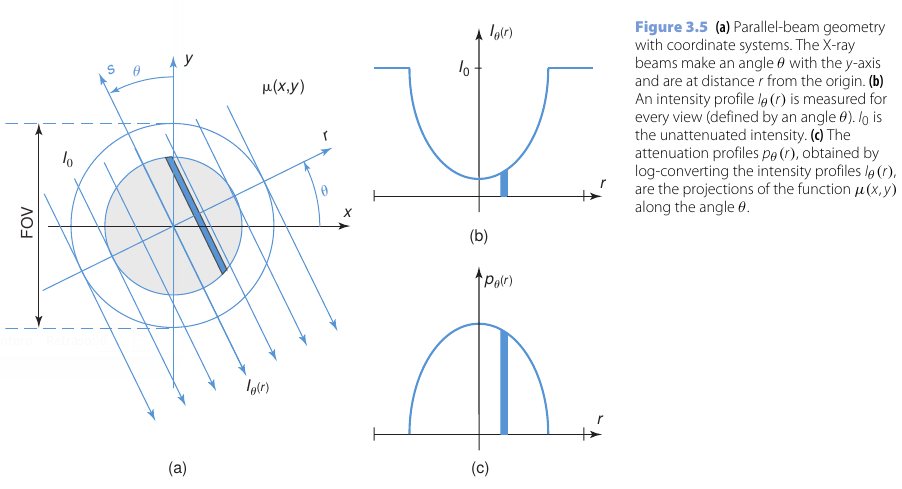
\includegraphics[width=.75\textwidth]{Figuras/cap10-1.png}
 \caption{}
 \label{fig:10-1}
\end{figure}

Entonces, para un ángulo $\theta$ dado, el perfil de intensidad $I_{\theta}(r)$ queda definido como

\begin{equation}
 I_{\theta}(r) = I_{0} \cdot e^{-\int_{L_{r,\theta}}\mu(x,y)ds} = I_{0} \cdot e^{-\int_{L_{r,\theta}}\mu(r\cdot \cos{\theta} - s\cdot \sen{\theta},r\cdot\sen{\theta} + s\cdot\cos{\theta})ds}
 \label{eq.10-4}
\end{equation}

\noindent
donde $L_{r,\theta}$ representa la línea que forma un ángulo $\theta$ con el eje $y$ a una distancia $r$ del orígen de coordenadas del sistema.

En términos realistas, tanto la atenuación como el espectro de rayos X dependen de la energía de los fotones, por lo que es necesario incorporar en la ecuación esta variable y la sección eficaz $\sigma(E)$. Pero en la práctica se asume un haz monocromático de energía $E_0$\footnote{Salvo la recientemente desarrollada técnica de \emph{dual-energy CT}.}.

Así, el perfil de atenuación $p_{\theta}(r)$ en función de $r$  se puede escribir a partir de la ec. \ref{eq.10-4} de la forma

\begin{equation}
 p_{\theta}(r) = -\ln{\left(\frac{I_{\theta}(r)}{I_0}\right)}
 \label{eq.10-5}
\end{equation}

donde $\pi_{\theta}(r)$ define la ``proyección'' de la función $\mu(x,y)$ a lo largo del ángulo $\theta$ y $p_{\theta}(r) = 0$ para $|r| \geq FOV/2$. Éste será medido en un

\subsection{Retroproyecci\'on}

\subsection{Teorema de la proyecci\'on}

\subsection{Reconstrucci\'on directa de Fourier}

\subsection{Retroproyecci\'on filtrada}

La retroproyección filtrada FBP\footnote{\emph{Filtered Back Projection}, por sus siglas en inglés.}

\subsection{Retroproyecci\'on filtrada en \emph{fan-beam}}

Hasta el momento solo se han considerado datos obtenidos de una configuración geométrica que asume haz paralelo desde la fuente pero, como hemos visto, los escaners de tercera y cuarta generación contemplan haces dispuestos en forma de abanico, también conocidos como \emph{fan-beam}.

Ahora, la ubicación $(x,y)$ que en el sistema de haz paralelo se ubicaba según el eje $(r,\theta)$, en fan-beam se indicará según los ejes $(\gamma, \beta)$, donde $\gamma$ es el ángulo entre el centro del abanico y la recta que une la fuente con $(x,y)$ y $\beta$ corresponde al ángulo entre la fuente y el eje $y$ (ver figura \ref{fig:10-2}). Se define además, el \emph{fan-angle} como el ángulo formado por el abanico. Ahora las mediciones deberán tomarse para $\beta$ entre 0 y $\pi$ + \emph{fan-angle}, para poder contemplar todas las regiones de interés. Por simplicidad, se asume entonces que el rango de los datos en $\beta$ será $(0, 2\pi)$.

\begin{figure}
 \centering
 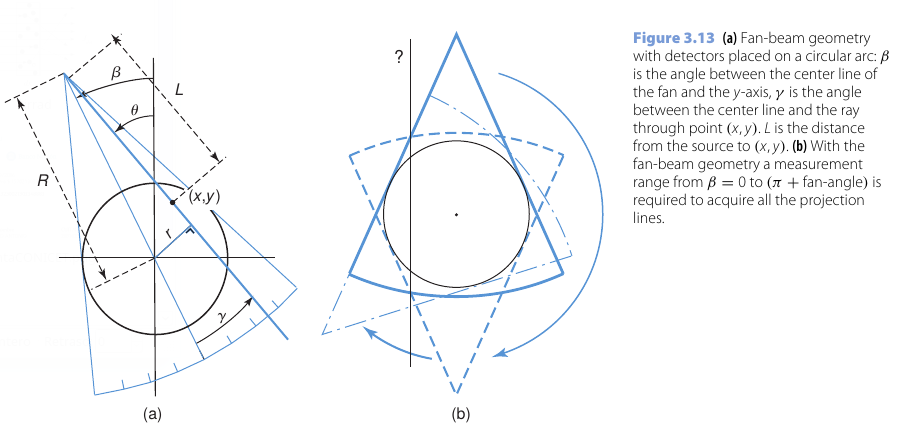
\includegraphics[width=.75\textwidth]{Figuras/cap10-2.png}
 \caption{}
 \label{fig:10-2}
\end{figure}

Los nuevos ejes $(\gamma, \beta)$ se corresponderán con los ejes $(r, \theta)$ según la transformación:

\begin{eqnarray}
 \theta = \gamma + \beta \\
 r = R \sen{\gamma}
\end{eqnarray}

\noindent
donde $R$ representa la distancia desde la fuente al centro del $FOV$. Tomando las ecuaciones de la FBP y limitando $r'$ a la integración en $[-FOV/2, FOV/2]$, se tiene que 

\begin{equation}
 f(x,y) = \frac{1}{2}\int_{0}^{2\pi}{\int_{-FOV/2}^{FOV/2}{p(r',\theta)\cdot q(x \cos{\theta} + y \sen{\theta} - r')dr'}d\theta}
\end{equation}

\noindent
donde $1/2$ se introduce solo para contemplar la integración sobre $(0, 2\pi)$ y dando lugar a 

\begin{equation}
 f(x,y) = \frac{1}{2} \int_{0}^{2\pi}{\int_{-\frac{fan-angle}{2}}^{\frac{fan-angle}{2}}{p(\gamma',\beta)\cdot q(x \cos{\gamma + \beta} + y \sen{\gamma + \beta} - R\sen{\gamma'})R \cos{\gamma'}d\gamma'}d\beta}
\end{equation}

\noindent
con lo que la fórmula para la reconstrucción en fan-beam resulta \cite{fundamentals2009}

\begin{equation}
 f(x,y) = \int_{0}^{2\pi} \frac{1}{L^{2}}\int_{-\frac{fan-angle}{2}}^{\frac{fan-angle}{2}}[R \cos{\gamma' \cdot p(\gamma', \beta)}] \cdot \frac{1}{2}\left(\frac{\gamma - \gamma'}{\sen{\gamma - \gamma'}}\right)^{2} q(\gamma - \gamma')d\gamma'd\beta
\end{equation}

\noindent
donde $L$ es la distancia entre la fuente y el punto $(x,y)$. Este resultado es visto como una expresión modificada de la FBP pesada por un factor $1/L^{2}$. La integral interna es la convolución de $p(\gamma, \beta)$, pesada por $R\cos{\gamma}$, con el kernel modificado $\frac{1}{2}(\gamma \sen{\gamma})^{2}q(\gamma)$.

Ecuaciones similares pueden obtenerse al considerar los detectores de forma lineal normales a la dirección del haz (ver figura \ref{fig:10-3}, obteniendo ahora una configuración de coordenadas $(t, \beta)$, donde $t$ es la distancia entre el origen y la recta que pasa por la fuente y el punto $(x, y)$. Ahora, el FBP pesado puede escribirse de la forma:

\begin{equation}
 f(x, y) = \int_{0}^{2\pi} \frac{1}{(U/R)^{2}}\int_{-\infty}^{+\infty}\left[\frac{R}{\sqrt{R^{2} + t'^{2}}}\cdot p(t', \beta)\right]\frac{1}{2}q(t-t')dt'd\beta
\end{equation}

\noindent
donde $U$ es la proyección de la distancia fuente-punto con el eje central del abanico.

\begin{figure}
 \centering
 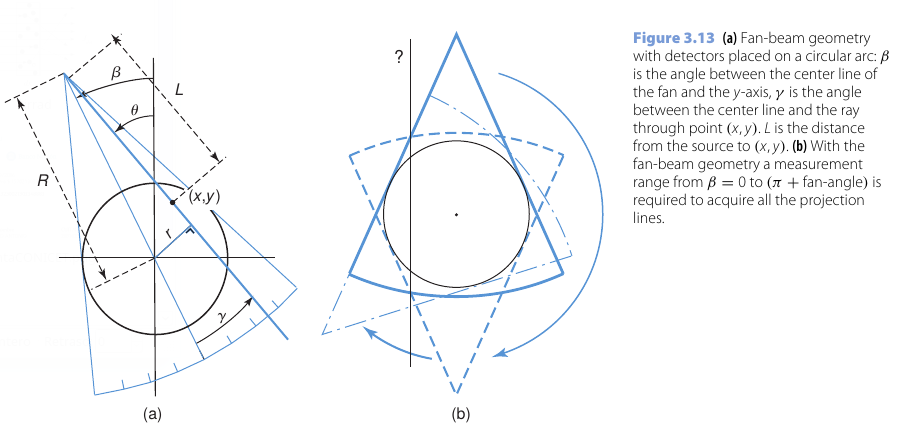
\includegraphics[width=.75\textwidth]{Figuras/cap10-2.png}
 \caption{}
 \label{fig:10-3}
\end{figure}

\subsection{Imagenes en 3 dimensiones}

\subsubsection{CT de un solo corte}

La forma de avanzar a la obtenci{\'o}n de una imagen tomogr{\'a}fica de un
determinado volumen consiste en escanear un n{\'u}mero de cortes consecutivos
por rotaciones circulares del tubo-detector alternando con peque{\~n}os
movimientos de la mesa donde se ubica el paciente. Esto es conocido como
escaneo axial. Para que este tipo de escaneo se pueda realizar sin perder
resoluci{\'o}n, es necesario satisfacer el criterio de Nyquist [cita]. La
distancia m{\'a}xima entre cortes consecutivos depende del ancho efectivo de
cada corte, com{\'u}nmente representado por el ancho total a la mitad del
m{\'a}ximo (FWHM) del perfil de sensitividad del corte (SSP) en el centro del
FOV. Si se asumen SSP rectangulares de ancho $\Delta z$, los datos deber{\'a}n
ser convolucionados con una funci{\'o}n bloque de ancho $\Delta z$. La
distancia m{\'a}xima entre dos cortes ser{\'a} entonces $\Delta z / 2$, con lo
que al menos se deben obtener dos cortes por ancho de corte.

Por otra parte, una de las t{\'e}cnicas m{\'a}s utilizadas en la actualidad es
la conocida como {\emph{CT helicoidal}} o {\emph{espiral}}\footnote{En
adelante se utilizar{\'a} el t{\'e}rmino {\emph{espiral}} para definir este
tipo de escaner. M{\'a}s all{\'a} que el t{\'e}rmino matem{\'a}tico m{\'a}s
apropiado es {\emph{helicoidal}}, el t{\'e}rmino {\emph{espiral}} se encuentra
m{\'a}s difundido para definir la t{\'e}cnica.}. En esta, el tubo de rayos X
rota cont{\'i}nuamente en torno al paciente, como en el caso de la CT 2D,
mientras la mesa se mueve de forma constante. Se conoce como {\emph{table
feed}} (TF) a la distancia recorrida por la mesa durante una rotaci{\'o}n
completa del tubo de 360$^{o}$. El {\emph{pitch}}, por otra parte, se
define como la raz{\'o}n entre TF y el espesor de un corte o
{\emph{slice}}\footnote{El uso de los t{\'e}rminos {\emph{corte}} y
{\emph{slice}} es indistinto en el texto.}.

En la CT circular, los datos son adquiridos a posiciones discretas en el eje
($z_1, z_2, \ldots, z_n$) y para posiciones
angulares del tubo entre 0 y 2$\pi$. Por otro lado, en la CT espiral los datos
son adquiridos mientras $\beta$ y $z$ crecen simult{\'a}neamente.

Asumiendo que uno desea reconstruir un slice en una posici{\'o}n determinada
del eje $z_1$ tomando la configuraci{\'o}n espiral, se necesitan datos de
$\beta$ barriendo el intervalo ($0, \pi + (\text{fan} - \text{angle})$) en
esta posici{\'o}n. Pero solo estar{\'a} disponible una vista a un {\'a}ngulo
$\beta^{\ast}$, problema que se resuelve por interpolaci{\'o}n de las
mediciones en las posiciones axiales adjacentes. Asumiendo SSP rectangulares
de ancho $\Delta z$ y siguiendo el mismo razonamiento que para CT circular,
llegamos a la conclusi{\'o}n de que la m{\'a}xima distancia de muestreo debe
ser $\Delta z / 2$. As{\'i}, para un ancho de slice $\Delta z$ tendremos un
TF$_{\max} = \Delta z / 2$ (pitch = 0.5). Finalmente, como los haces opuestos
producen la misma informaci{\'o}n, la distancia the muestreo resulta TF/2 y la
m{\'a}xima TF = $\Delta z$ (pitch = 1). Incrementar el pitch para valores > 1
reducir{\'a} el tiempo de escaneo, pagando un costo en la calidad de la
imagen. Te{\'o}ricamente, por esto, la dosis en el paciente se reduce al
incrementarse el valor del pitch, pero esto no sucede en la pr{\'a}ctica pues
se mantiene constante al incrementarse los $\text{mAs}$ para mantener la CNR
que determina la calidad de la imagen.

\subsubsection{CT multi-slice}

En los esc{\'a}ners modernos, los arreglos de detectores consisten
m{\'u}ltiples columnas de detectores, con el objetivo de medir varios cortes
por rotaci{\'o}n del tubo de rayos X. En este caso el pitch puede ser definido
como la raz{\'o}n entre el TF respecto del total del ancho del haz de rayos X.
Como en los casos anteriores, utilizando el mismo valor de pitch se obtiene
una reducci{\'o}n del tiempo de escaneo dada por el n{\'u}mero de columnas de
detectores, resultando en una disminuci{\'o}n de artefactos producidos por el
movimiento del paciente.

Si la distancia entre la fuente y los detectores es lo suficientemente grande,
todas las l{\'i}neas pueden asumirse como paralelas y el problema se reduce al
de la reconstrucci{\'o}n de una serie de im{\'a}genes 2D. Suele suceder cuando
hay 4 columnas de detectores adyacentes, pero esta asumpci{\'o}n ya no puede
ser asumida para esc{\'a}ners de 16 cortes. Una aproximaci{\'o}n a la
soluci{\'o}n de este problema, consiste en inclinar cada imagen planar de
forma tal de minimizar su distancia media a las posiciones de la fuente
involucradas en la reconstrucci{\'o}n del plano. Despu{\'e}s de la
reconstrucci{\'o}n 2D de los planos inclinados, los cortes axiales se logran
por interpolaci{\'o}n. Esta t{\'e}cnica es conocida como
{\emph{reconstrucci{\'o}n de plano inclinado}}.

A medida que el n{\'u}mero de columnas de detectores crece, aparecen m{\'a}s
artefactos en la reconstrucci{\'o}n, por lo que en ese caso se deben
implementar m{\'e}todos de reconstrucci{\'o}n 3D directos ({\emph{fully 3D
reconstruction}}). En los escaners multi slice el operador cuenta con la
posibilidad de especificar el espesor de cada corte, m{\'a}s all{\'a} del
ancho de los detectores. Los slices m{\'a}s gruesos tienen un SNR m{\'a}s
alto. {\'E}stos pueden ser obtenidos por convoluci{\'o}n de los valores de las
proyecciones medidas a lo largo del eje $z$ con un filtro de suavizado, y la
t{\'e}cnica es conocida como {\emph{z-filtering}}.

\subsubsection{CT volum{\'e}trica}

Un volumen completo puede incluso ser obtenido en un solo giro del tubo de
rayos X, aunque para lograrlo es necesario un haz c{\'o}nico muy grande. En
este caso, y en el resto salvo el de haces paralelos, se requiere una
reconstrucci{\'o}n 3D.

En 3 dimensiones, el terorema de la proyecci{\'o}n establece que la
transformada de Fourier 3D de una funci{\'o}n en la direcci{\'o}n $\vec{k}$ es
igual a la transformada de Fourir en 1 dimensi{\'o}n a lo largo de la misma
direcci{\'o}n de las integrales del plano perpendicular a esa direcci{\'o}n.
El teorema de la proyecci{\'o}n provee una soluci{\'o}n matem{\'a}tica a la
real reconstrucci{\'o}n 3D en los casos donde las trayectorias de las fuentes
son suficientes como para proveer integrales planares y donde no hay
truncamiento en el detector. El escanning t{\'i}pico utilizado en la
pr{\'a}ctica cl{\'i}nica es el circular y el helicoidal.

\paragraph{Reconstrucci{\'o}n circular en haz c{\'o}nico}

En el caso de las trayectorias circulares, es imposible te{\'o}ricamente la
reconstrucci{\'o}n volum{\'e}trica excepto para v{\'o}xeles o semi-planos, ya
que no se posee suficiente informaci{\'o}n de las mediciones. Por esto se
utiliza un algoritmo de reconstrucci{\'o}n aproximado. El m{\'a}s famoso es el
conocido como FDK, propuesto por Feldkamp en 1984, que extiende el FBP en 2D a
3 dimensiones
\[ f (x, y, z,) = \int_0^{2 \pi} \frac{1}{(U / R)^2} \int_{- \infty}^{\infty}
   \left[ \frac{R}{\sqrt{R^2 + t'^2} + \zeta^2} \cdot p (t', \zeta, \beta)
   \right] \cdot \frac{1}{2} q (t - t') \text{dt}' d \beta \]
donde $\zeta$ es la altura del abanico inclinado sobre la rotaci{\'o}n del
centro de la fuente y $U$ es la proyecci{\'o}n de la distancia fuente-punto en
el rayo central del abanico no-inclinado.

Como el algoritmo solo ofrece aproximaciones, los artefactos debidos al haz
c{\'o}nico son inevitables.

\paragraph{Reconstrucci{\'o}n helicoidal en haz c{\'o}nico}

A diferencia del caso anterior, en este caso se posee toda la informaci{\'o}n
necesaria para una reconstrucci{\'o}n directa cuando pitch $\leq 1.3$. La
aproximaci{\'o}n DBP\footnote{{\emph{Derivative back-projection}}, por sus
siglas en ingl{\'e}s.} provee una reconstrucci{\'o}n precisa para estos casos.
Sin embargo, por la falta de algoritmos exactos para esta reconstrucci{\'o}n,
la mayor{\'i}a de los fabricantes utiliza algoritmos aproximados como el FDK
que son preferibles en t{\'e}rmios del ruido, la uniformidad del ruido y otras
caracter{\'i}sticas que afectan la calidad.

\paragraph{Reconstrucci{\'o}n iterativa}

Como es usado sobre todo en PET y SPECT, la reconstrucci{\'o}n iterativa se ha
incorporado recientemente a los escaners comerciales. Esto se ha hecho
recientemente porque la capacidad computacional para el procesamiento no era
compatible con el hardware disponible a{\~n}os atr{\'a}s. La discusi{\'o}n de
los algoritmos iterativos no se encuentra dentro de los objetivos de este
texto, por lo que solo se menciona a fines de completitud.



\section{Aplicaciones en radiodiagn\'ostico metab\'olico: PET y SPECT}

\section{Nociones y requerimientos de matching y fusi\'on de im\'agenes anat\'omicas y metab\'olicas}